

\section{Main input file (CON file format)}
\label{sec:CONformat}

\begin{figure}
 \begin{center}
 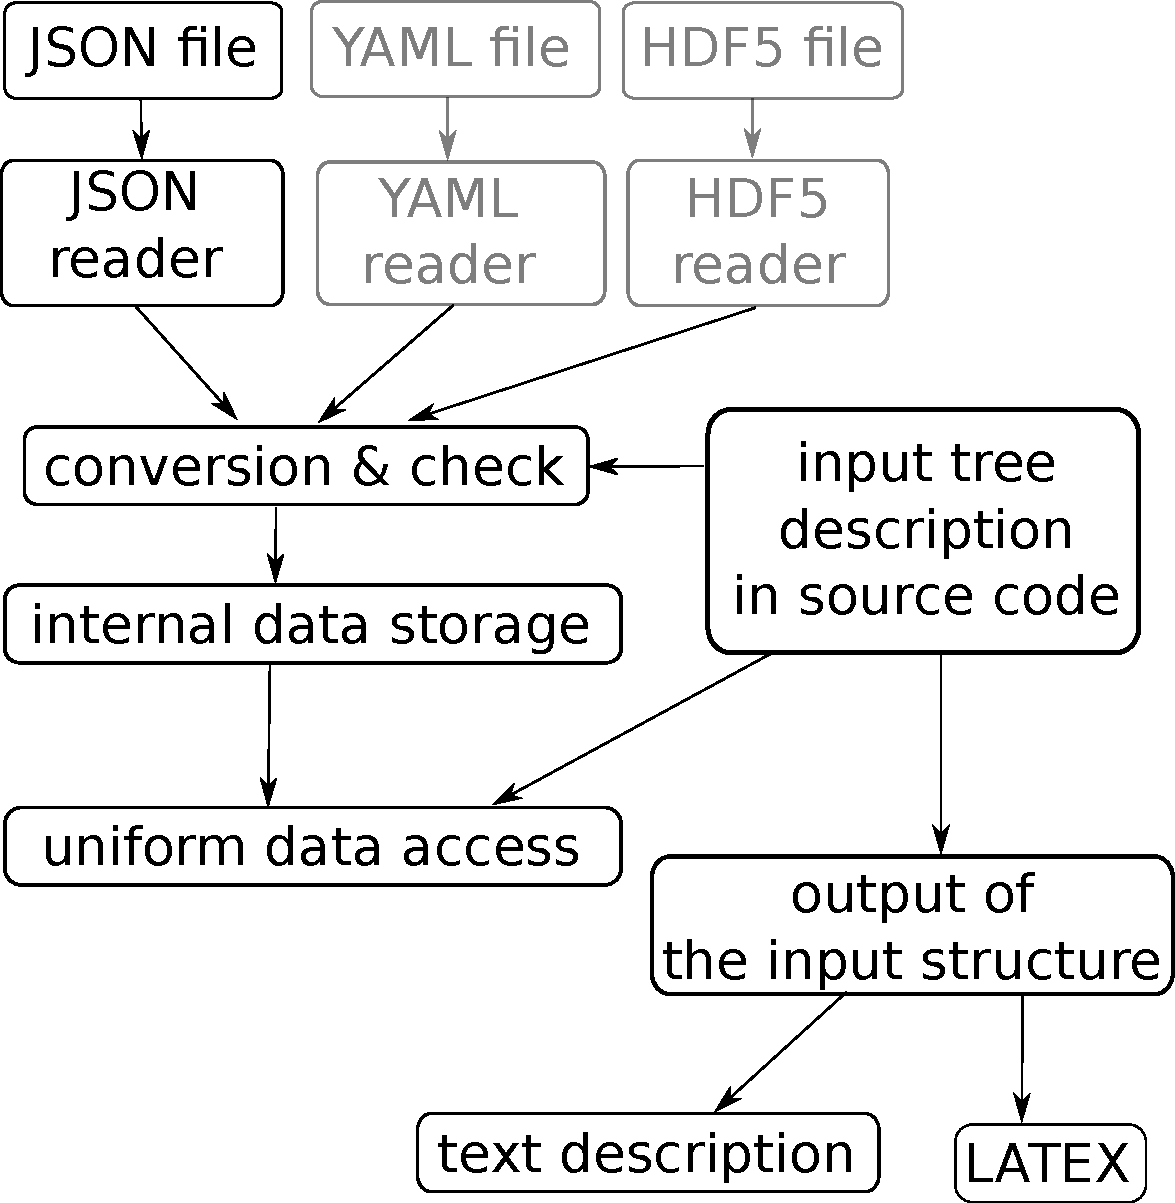
\includegraphics[scale=0.4]{./input_subsystem.pdf}
 % input_subsystem.pdf: 0x0 pixel, -2147483648dpi, 0.00x0.00 cm, bb=
 \caption{Sturucture of the input subsystem. Grey boxes are not implemented yet.}
 \label{fig:input_subsystem}
 \end{center}
\end{figure}

In this section, we shall describe structure of the main input file that is given through the parameter \verb'-s' on the command line.
The file formats of other files that are referenced from the main input file and used for input of the mesh or large field data
(e.g. the GMSH file format) are described in following sections. The input subsystem was designed with the aim to provide uniform initialization of 
C++ classes and data structures. Its structure is depicted on Figure \ref{fig:input_subsystem}.
The structure of the input is described by the Input Types Tree (ITT) of (usually static) objects which follows the structure of the classes.
The data from an input file are read by apropriate reader, their structure is checked against ITT and they are pushed into the Internal Storage Buffer (ISB).
An accessor object to the root data record is the result of the file reading. The data can be retrieved through accessors which combine 
raw data stored in in IBS with their meaning described in ITT. ITT can be printed out in various formats providing description of the input structure both for 
humans and other software.

Currently, the JSON input file format is only implemented and in fact it is slight extension of the JSON file format. On the other hand
the data for initialization of the C++ data structures are coded in particular way. Combination of this extension and restriction of the JSON file format produce 
what we call CON (C++ object notation) file format.


\subsection{JSON for humans}

Basic syntax of the CON file is very close to the JSON file format with only few extensions, namely:
\begin{itemize}
\item You can use C++ (or JavaScript) comments. One line comments \verb'//' and multi-line comments \verb'/* */'.
\item The quoting of the keys is optional if they do not contain spaces (holds for all CON keys).
\item You can use equality sign \verb'=' instead of colon \verb':' for separation of keys and values in JSON objects.
\item You can use any whitespace to separate tokens in JSON object or JSON array.
\end{itemize}
The aim of these extensions is to simplify writing input files manually. However these extensions can be easily filtered out and converted to 
the generic JSON format. For the description of the JSON format we refer to \url{http://www.json.org/}. 

\subsection{CON constructs}
The CON file format constructs are designed for initialization of C++ strongly typed variables. The primitive data types can be initialized from 
the primitive CON constructs: 
\begin{itemize}
 \item {\it Bool} --- initialized from the JSON keywords \verb'true' and \verb'false'.
 \item {\it Double}, {\it Integer} --- initialized from JSON numeric data. 
 \item {\it String}, {\it FileName}, {\it Selections} --- initialized from JSON strings
\end{itemize}
Selections are typed like the C++ enum types that are initialized from them.
Various kind of containers can be initialized by the {\it Array} construct, that is an JSON array with elements of the same CON type. 
The C++ structures and classes can be initialize from the {\it Record} construct, which is represented by a JSON object. However, in constrast to JSON,
these Records have different types in similar way as the strong typed C++ structures. The types are described by ITT of the particular program
which can be printed out in several formats, in particular description of ITT for Flow123d forms content of Chapter \ref{chapter:input-tree-reference}.
In order to allow certain kind of polymorphism, we introduce also the {\it AbstractRecord} construct, where the type of the record is not given by ITT but 
can be chosen as part of the input. 

\subsection{CON special keys}
All keys in Records should be in lower case, possibly using digits and underscore. The keys all in upper case are reserved for special function in the 
CON file. These are:
\begin{description}

\item[TYPE key]:
\begin{verbatim}
TYPE=<Selection of AbstractRecord>
\end{verbatim}
Is used to specify particular type of an AbstractRecord. This way you can choose which particular implementation of an abstract C++ class should be instantiated.
The value of the key is a string from the Selection that consists of names of Records that was declared as descendants of the AbstractRecord.


%\item[INCLUDE\_RECORD]:\\
%This is a simple inclusion of another file as a content of a record:
%\begin{verbatim}
%{
%        INCLUDE_RECORD = "<file name>"
%}
%\end{verbatim}
%
%\item[INCLUDE\_ARRAY]:\\
%\begin{verbatim}
%array=
%{
%        INCLUDE_ARRAY = "<file name>"
%        FORMAT = "<format string>"
%}       
%\end{verbatim}
%The reader will substitute the include record by a sequentially accessible array. The file has fixed number of 
%space separated data fields on every line. Every line becomes one element in the array of type record. Every line forms a 
%record with key names given by the \verb'<format string>' 
%and corresponding data taken form the line.

%The key difference compared to regular JSON arrays is that included arrays can be accessed only sequentially 
%within the program and thus we minimize reader memory overhead for large input data. The idea is to translate raw data into structured
%format and use uniform access to the data.

%Basic syntax for format string could be an array of strings --- formats of individual columns.
%Every format string is an address of key that is given the column. Onother possibility is to give an arbitrary 
%JSON file, where all values are numbers of columns where to take the value.

%[\dots better specify format string]


%Possible extensions:
% have sections in the file for setting time dependent data
% have number of lines at the beginning
% have variable format
% allow vectors in the 'line records']

\item[REF key]:
\begin{verbatim}
{ REF=<address> }
\end{verbatim}
The record in input file that contains only the key \verb'REF' is replaced by the JSON entity that is referenced by the \verb'<address>'. 
The address is a string with format similar to UNIX path, i.e. with grammar
\begin{verbatim}
    <address> = <address> / <item>
              = <item>  
              = <null>
    <item> = <index>
           = <key>
           = ..
\end{verbatim}
where \verb'index' is non-negative integer and key is valid CON record key (lowercase, digits, underscores).
The address can be absolute or relative identification of an entity. The relative address is relative to the entity in which the reference record is contained.
One can use two dots \verb'".."' to move to parent entity.

Example:
\begin{verbatim}
mesh={
        file_name="xyz"
}
array=[
        {x=1 y=0}       
        {x=2 y=0}
        {x=3 y=0}
]               
outer_record={
        output_file="x_out"
        inner_record={
                output_file={REF="../output_file"} // value "x_out"
        }
        x={REF="/array/2/x"}                       // value "3"
        f_name={REF="/mesh/file_name"}             // value "xyz"
}       
\end{verbatim}
\end{description}

\subsection{Record types}
A Record type is given by the set of key specifications, which in turn consist from: key name, type of value and default value specification.
Default value specification can be:
\begin{description} 
 \item[obligatory] --- means no default value, which has to be specified at input. 
 \item[optional] --- means no default value, but value is needs not to be specified. Unspecified value usually means that you turn off some functionality.
 \item[default at declaration] --- the default value is explicitly given in declaration and is automatically provided by the input subsystem if needed
 \item[default at read time] --- the default value is provided at read time, usually from some other variable. In the documentation, 
 there is only textual description where the default value comes from.
\end{description}

\subsubsection{Implicit creation of composed entities}
Consider a Record type in which all keys have default values (possibly except one). Then the specification
of the Record can contain a {\it key for default construction}. User can specify only the value of this particular key instead of the whole record, all other keys are initialized from its default values.
Moreover, an AbstractRecord type may have a default value for the \verb'TYPE' key.
This allows to express simple tasks by simple inputs but still make complex inputs possible. 
Similar functionality holds for arrays. If the user sets a non-array value where an array is expected the reader provides an array with a unique element holding the given value.


\section{Important Record types of Flow123d input}


\subsection{Mesh record}
\label{sec:Mesh}
The \hyperlink{IT::Mesh}{mesh record} provides initialization for the computational mesh consisting of points, lines, triangles and tetrahedrons in 3D space.
Currently, we support only GMSH mesh file format \href{http://geuz.org/gmsh/doc/texinfo/gmsh.html#MSH-ASCII-file-format}{MSH ASCII}. 
The input file is provided by the key \hyperA{Mesh::mesh-file}{{\tt mesh\_file}}. The file format allows to group elements into {\it regions} identified either by ID number or by string label. 
The regions with labels starting with the dot character are treated as {\it boundary regions}. Their elements are removed from the computational domain, however they can be used to specify boundary
conditions. Other regions are called {\it bulk regions}. User can create new labeled regions through the key 
\hyperA{Mesh::regions}{{\tt regions}}, the new region can be specified either by its ID
or by list of IDs of its elements. The latter possibility overrides original region assigned to the elements, which can be useful for specification of small areas ``ad hoc''.
The key \hyperA{Mesh::sets}{{\tt sets}} allows specification of sets of regions in terms of list of region IDs or labels and basic set operations. The difference between regions and sets is that
regions form disjoint covering of elements, the sets, however, may overlap. There are three predefined region sets: ``ALL'', ``BOUNDARY'', ``BULK''.


\subsection{Field records}
\label{}
A general time and space dependent, scalar, vector, or  tensor valued function can be specified through the family of abstract records 
Field $R^m -> \mathcal{S}$, where $m$ is currently always $m=3$ and $\mathcal{S}$ is a specification of the target space, which can be:
\begin{itemize}
 \item {\bf $\mathcal{T}$} --- scalar valued field, with scalars of type $\mathcal{T}$
 \item {\bf $\mathcal{T}[d]$} --- vector valued field, with vector of fixed size $d$ and elements of type $\mathcal{T}$
 \item {\bf $\mathcal{T}[\tt n]$} --- vector valued field, with vector of variable size (given by some input) and elements of type $\mathcal{T}$
 \item {\bf $\mathcal{T}[d, d]$} --- tensor valued field, with square tensor of fixed size and elements of type $\mathcal{T}$
\end{itemize}
the scalar types can be
\begin{itemize}
 \item {\bf Real} --- scalar real valued field
 \item {\bf Int}  --- scalar integer valued field
 \item {\bf Enum} --- scalar non negative integer valued field, should be convertible to appropriate C++ enum type
\end{itemize}

Each of these abstract record has the same set of descendants which implement various algorithms to specify and compute values of the field. These are
\begin{description}
 \item[FieldConstant] --- field that is constant in space
 \item[FieldFormula] --- field that is given by runtime parsed formula using $x,y,z,t$ coordinates. The \href{http://warp.povusers.org/FunctionParser/}{Function Parser} library is used
 with syntax rules described \href{http://warp.povusers.org/FunctionParser/fparser.html#literals}{here}.
 \item[FieldPython] --- field can be implemented by Python script either specified by string (key \hyperA{FieldPython::script-string}{{\tt script\_string}}) 
 or in external file (key \hyperA{FieldPython::script-file}{{\tt script\_file}}. 
 \item[FieldElementwise] --- discrete field, currently only piecewise constant field on elements is supported, the field can given by 
 the \href{http://geuz.org/gmsh/doc/texinfo/gmsh.html#MSH-ASCII-file-format}{MSH ASCII} file specified in key \hyperA{FieldElementwise::gmsh-file}{{\tt gmsh\_file}} and field name in the file given 
 by key \hyperA{FieldElementwise::field-name}{{\tt field\_name}}. The file must contain same mesh as is used for computation.
 \item[FieldInterpolated] --- allows interpolation between different meshes. Not yet fully supported.
\end{description}

Several automatic conversions are implemented. Scalar values can be used to set constant vectors or tensors. Vector value of size $d$ can be used to set diagonal tensor $d\times d$.
Vector value of size $d(d-1)/2$, e.g. $6$ for $d=3$, can be used to set symmetric tensor. These rules apply only for FieldConstant and FieldFormula.
Moreover, all Field abstract types have default value \verb'TYPE=FieldConstant'. Thus you can just use the constant value instead of the whole record.

Examples:
\begin{verbatim}
constant_scalar_function = 1.0
// is same as
constant_scalar_function = {
  TYPE=FieldConstant,
  value=1.0
}

conductivity_tensor = [1 ,2, 3]
// is same as
conductivity_tensor = {
    TYPE=FieldConstant,
    value=[[1,0,0],[0,2,0],[0,0,3]]
}

concentration = {
    TYPE=FieldFormula,
    value="x+y+z"
}
//is same as (provided the vector has 2 elements)
concentration = {
    TYPE=FieldFormula,
    value=["x+y+z", "x+y+z"]
}       
\end{verbatim}

\subsection{Field data for equations}
Every equation record has keys \verb'bulk_data' and \verb'bc_data'. Both have the same structure, however, the first one is intended to set the bulk fields (on bulk regions)
while the second serves for initialization of the boundary fields (on boundary regions). These keys contains an array of region-time initialization records
like the \hyperlink{IT::DarcyFlowMH-Steady-BulkData}{BulkData} record of the DarcyFlow equation. Every such record specify fields on particular region 
(keys \hyperA{DarcyFlowMH-Steady-BulkData::region}{{\tt region}} and \hyperA{DarcyFlowMH-Steady-BulkData::rid}{{\tt rid}} ) or on a region set 
(key \hyperA{DarcyFlowMH-Steady-BulkData::r-set}{{\tt r\_set}}) starting from the time specified by the key \hyperA{DarcyFlowMH-Steady-BulkData::time}{{\tt time}}.
The array is processed sequentially and latter values overwrites the previous ones. Times should form a non-decreasing sequence.

Example:
\begin{verbatim}
bulk_data = [   
    { // time=0.0  - default value
        r_set="BULK"
        conductivity=1   // setting the conductivity field on all regions
    }
    {
        region="2d_part"
        conductivity=2  // overwriting the previous value
    }
    {   time=1.0
        region="2d_part"
        conductivity={
            // from time=1.0 we switch to the linear function in time
            TYPE=FieldFormula
            value="2+t"      
        }    
    }
    {   time=2.0
        region="2d_part"
        conductivity={
            // from time=2.0 we switch to elementwise field, but only
            // on the region "2d_part"
            TYPE=FieldElementwise
            gmsh_file="./input/data.msh"
            field_name="conductivity"
        }
    }    
]               
\end{verbatim}

